\chapter{Rendszer megvalósítása}

\begin{figure}[H]
	\centering
	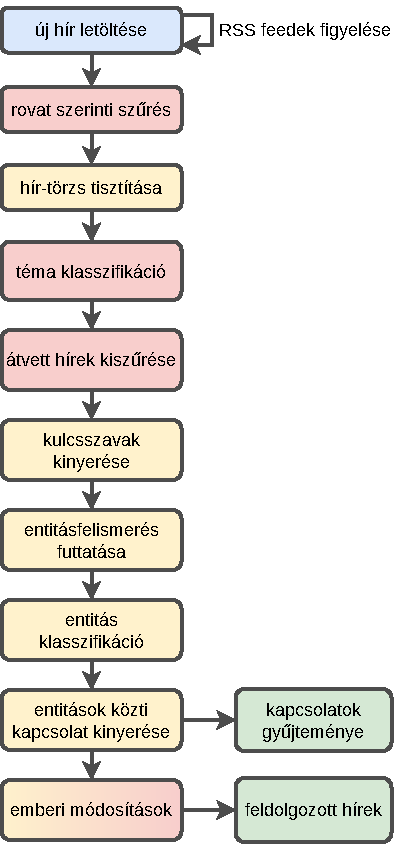
\includegraphics[width=80mm,keepaspectratio]{figures/flowchart-konkret.pdf}
	\caption{Rendszer működését bemutató folyamatábra}
\end{figure}

\section{Rendszer összeállítása}

Mivel a szoftver-rendszer több különálló modell összekapcsolásával működik adta magát a modulokra bontás. A konténerizáláshoz Docker-t használtam, összesen hat darab konténer dolgozik a rendszer feladatainak ellátásáért.

Egy fő konténer futtatja a webszervert, figyeli a cikkek megjelenését, előszűri a cikkeket és a szövegek előtisztítását is elvégzi. A finomhangolt BERT modell egy külön konténerben fut \texttt{transformers} könyvtár segítségével további optimalizáció nélkül. A névelemek detektálását végző HuSpaCy szintén egy külön konténerből szolgálja ki a fő konténer kéréseit. A három finomhangolt GPT modell mindegyike saját konténerben fut.

A modulok közti kommunikáció REST API-okon keresztül folyik, amihez vegyesen FastAPI és Flask Python könyvtárt használtam.

\subsection{Modellek felkészítése telepítésre}

A Mistral-ból finomhangolt modelleket llama.cpp segítségével sikerült optimális módon futtatnom videokártya nélkül. Ehhez viszont szükség volt a modellek \texttt{gguf} formátumra való konvertálására, mivel a llama.cpp által használt \texttt{ggml} könyvtár ezt követeli meg.

A nagy nyelvi modellek futtatása erőforrás használat és teljesítmény szempontjából is optimalizálható a modellek kvantálásával, mindezt a minőség nagy részének megtartása mellett. A modellek mindegyikéhez \texttt{Q4\_K\_M} kvantálást használtam, ami 7 milliárd paraméteres modelleke esetében egy optimális középút a teljesítmény és a pontosság között.

\subsection{Webes felület}

A rendszer kimenetének felülvizsgálása érdekében fejlesztettem egy webes felületet, amivel az elemzett hírek egyszerűen szerkeszthetők. A felület összeállításához backend-en Flask keretrendszert használtam. Mivel az adatok mentésében a konkurencia nem jelent kihívást, ezért egy nagyszabású adatbázis helyett egyszerűen \texttt{sqlite}-ot használtam adattárolásra.

\begin{figure}[H]
	\centering
	\subfloat[\centering Hírek listája]{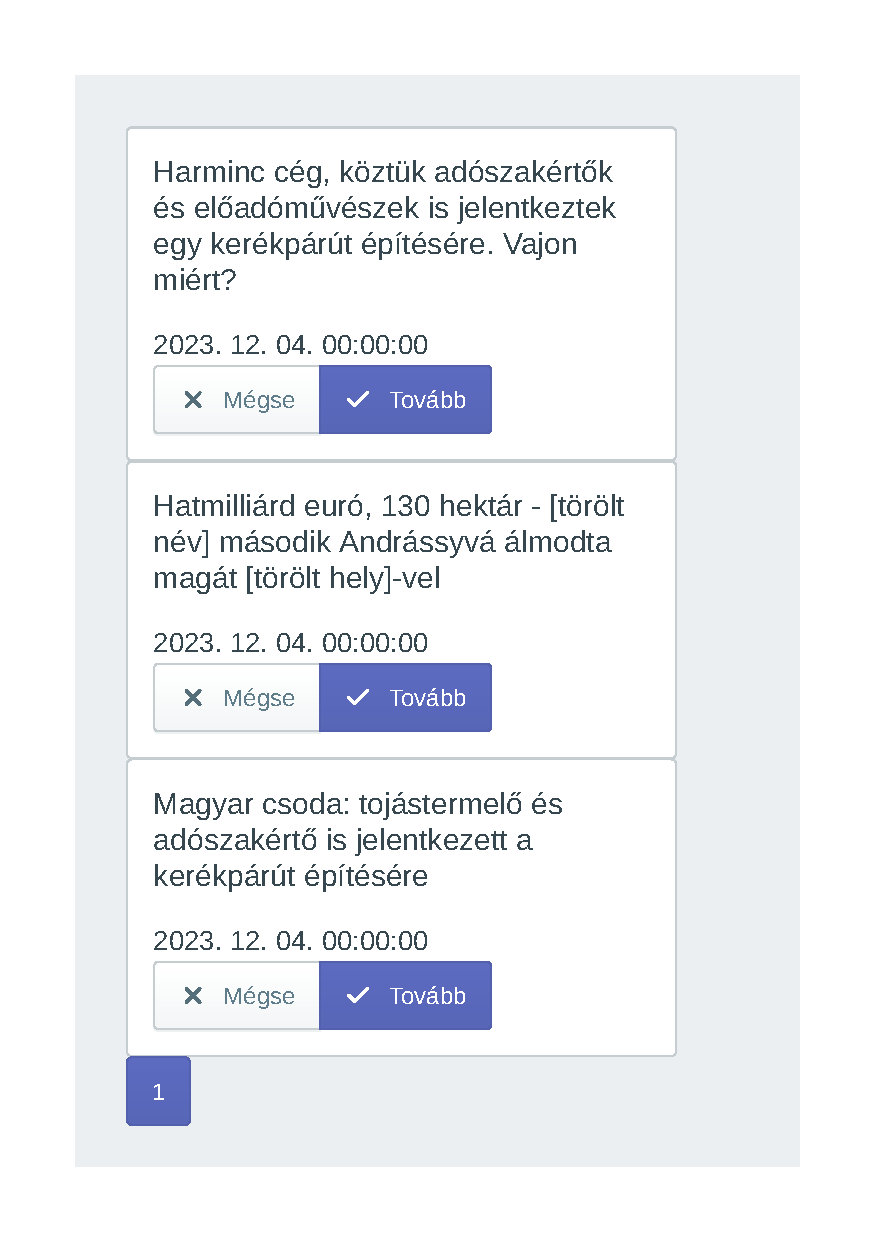
\includegraphics[width=.45\linewidth,keepaspectratio]{figures/kmdb-webapp-list.pdf}}
	\qquad
	\subfloat[\centering Hír szerkesztése]{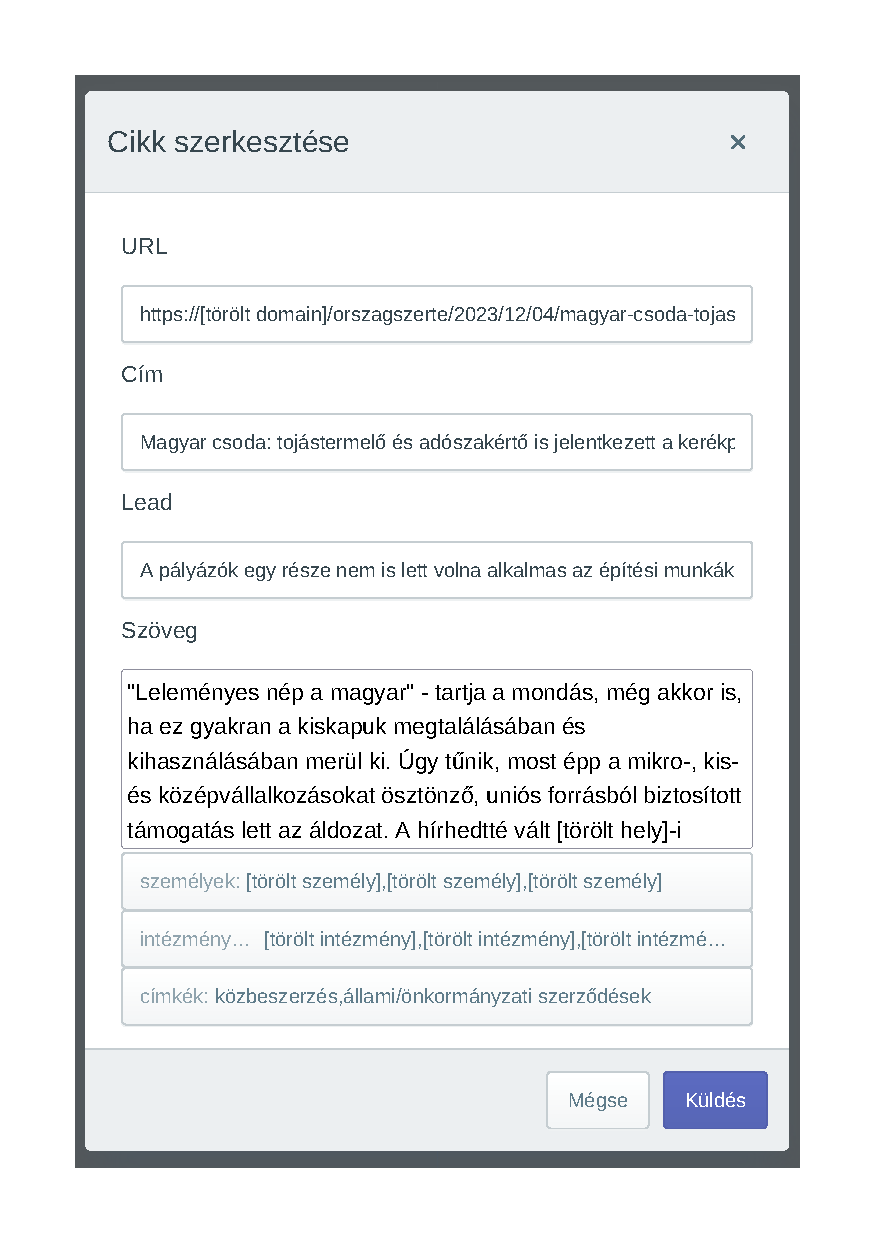
\includegraphics[width=.45\linewidth,keepaspectratio]{figures/kmdb-webapp-edit.pdf}}
	\caption{Webes felület}%
	\label{fig:webui}%
\end{figure}

A frontend elkészítéséhez egy alacsony erőforrásigényű keretrendszert választottam, a \texttt{Mithril.js}-t. Emellett a UI elemek jelentős részét a keretrendszerhez fejlesztett \texttt{construct-ui}-ból kölcsönöztem.
